\documentclass{article}

\usepackage{caption} 
\captionsetup[table]{skip=10pt}
\usepackage{arxiv}
\usepackage{graphicx}
\usepackage{amsmath}
\usepackage{float}
\usepackage{subfig}
\usepackage[utf8]{inputenc} % allow utf-8 input
\usepackage[T1]{fontenc}    % use 8-bit T1 fonts
\usepackage{hyperref}       % hyperlinks
\usepackage{url}            % simple URL typesetting
\usepackage{booktabs}       % professional-quality tables
\usepackage{amsfonts}       % blackboard math symbols
\usepackage{nicefrac}       % compact symbols for 1/2, etc.
\usepackage{microtype}      % microtypography
\usepackage{lipsum}

\title{BBM-497 Assignment 1}


\author{
  Hakan AKYÜREK \\
  \texttt{b21426553@cs.hacettepe.edu.tr} \\
  %% examples of more authors
}

\begin{document}
\maketitle

\section{Introduction}
In this report I discuss my approaches to given tasks, namely author detection and essay generation, my approach to language model structure, and analysis of results.
\section{Language Model}

I used a Bag of Words(BoW) model for the tasks. I have trained 3 for each author, 6 in total, models, which are all able to both generate an essay and return a probability for an given essay. They are all saved as pickle files under the models folder under project root.

Finding a proper way to store and access the data in the model was a problem. To solve it, I created a dictionary where the keys are condition words and the values are count and another dictionary, namely next. In the inner dictionary, next, each word that come after the condition words are stored as keys and their counts are stored as their values. The count on the outer scope is the sum of all of them.

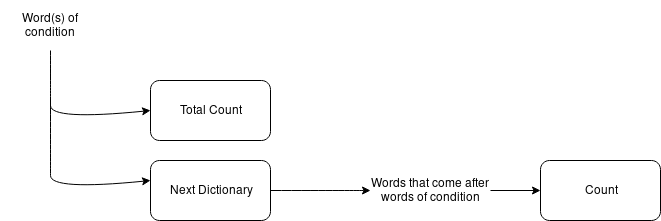
\includegraphics[width=1\linewidth, height=5cm]{asdf}

The structure above lets me to access data required in $O(1)$, while rescues me from the unnecessary memory usage like it would happen in a matrix.

Language Models follow the same equations for both essay generation and author detection, where n is equal to n-gram number:
\begin{gather}
n > 1: P(sentence) = \prod_{k=1}^mP(W_k | W_{k-1} W_{k-2} ... W_{k-n-1}) \\
n = 1: P(sentence) = \prod_{k=1}^mP(W_k)
\end{gather}

To avoid underflow and harder calculations, I work on a log space with these probabilities:
\begin{gather}
n > 1: P(sentence) = \sum_{k=1}^mlog(P(W_k | W_{k-1} W_{k-2} ... W_{k-n-1})) \\
n = 1: P(sentence) = \sum_{k=1}^mP(W_k)
\end{gather}

There may be also out of vocabulary words in test dataset. To avoid various errors I needed to use Laplace smoothing on probability calculations, such as the bi-gram equation below:

\begin{equation}
n = 2:
P(W | W_{k-1}) = \frac{C(W_{k-1}, W_k) + 1}{C(W_{k-1}) + V}
\end{equation}

where V is the number of the unique keys in models dictionary, namely condition words.
\subsection{Essay Generation}

In essay generation I forced my models to generate an essay with only 30 words maximum. Any tokens or punctuations aren't considered a word in the essays. I have used the next dictionary to quickly get the counts of next words after condition words in bi and tri-gram models. In uni-gram models I did not need to use the next dictionary at all since it is unnecessary to generate a essay with uni-gram.

The work-flow of generation is rather simple, an example with bi-gram is given below:
\begin{itemize}
\item[1.] Put one start token to beginning since n is 2.
\item[2.] Calculate the probabilities of the next words coming after the current word using equation 5.
\item[3.] Scale all of the probabilities to 1 and put them in an array.
\item[4.] Generate a random float between 0 and 1 and select the next word.
\item[5.] Repeat steps 2-4 until the end.
\end{itemize}

\begin{center}
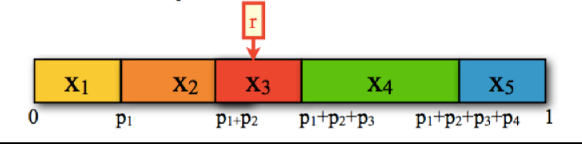
\includegraphics[width=0.7\linewidth, height=2cm]{essay}
\end{center}

\subsection{Author Detection}

In author detection the goal was to calculate the probability of the essays with both n-gram models using equations 3 or 4. Then the program picks the higher probability as the prediction of the author.
\section{Dataset}

There are some number of modifications to dataset in order to process it better. Firstly, I have filtered punctuations, except quotes, to have a white-space between the words around them. The main reason of that is I wanted to count them as separate tokens in my model. After that I put '\texttt{\_START\_}' and '\texttt{\_END\_}' tokens to start and end of all documents and also before and after every separated punctuation. Accordingly, by putting the end token my models actually learned which words end a sentence and which do not, so it can use a word, which was used before a comma, before a point to end a sentence. Similarly, with the start token my models can learn which words can start a sentence.

Furthermore, I have also reduced the number of words in the dictionary by shortening phrases like 'I am', 'You were not', ' He would not'. Accordingly, this helped me to reduce the complexity and get better results in both tasks. Additionally, all data is represented in lower-case except start and end tokens to again decrease the number of words in the dictionary.

\section{Results}
My results in essay generation are nothing surprising. Uni-gram models generate completely garbage essays, while bi-gram models generate a little bit better tri-gram models are superior than bi-gram models in that respect. More essays can be found in 'essays.txt' in root folder of the project.

Uni-gram model:
\begin{quote}
. representatives the . for should fellowcitizens be . once security in ; resides relief , ; states , less are than it so legal states enterprising pointed the . , constitution , lain which and particular which be retrospective
\end{quote}

Bi-gram model:
\begin{quote}
that this quarter of the immediate interest , not likely to the legislative and of the sources from an overcurious discussion and consuls into foreign jurisdiction left in each other
\end{quote}

Tri-gram model:
\begin{quote}
therefore , for the twelve states . besides other impediments , which supposes a pre-existing government of a particular state , taxes on articles imported from other circumstances ; if
\end{quote}
Although what the latter models generate are somewhat meaningful, because of the randomness the topic of start and  end of the sentences do not match at all. Models remembering at most 2 words while generating is also a factor. We can also see in uni-gram there are loads of punctuations generated, while in bi and tri-gram models number of punctuations are severely reduced. We can also see in uni-gram model doesn't know what words should be at the start and which words should be at the end. This also makes uni-gram generations completely meaningless.

The results of articles 9, 11, 12, 47, 48, 58 are represented in Table 1. The results show us that the tri-gram models are also superior than others when classifying documents. While uni-gram models fail to label Hamilton's articles they are still able to label Madison's correctly. It seems that uni-gram is unable to get any semantic meaning out of the articles and Madison's usage of punctuations increase her probability scores. Because when I switch to bi-gram it correctly classify 2 of Hamilton's articles.

\begin{table}[H]
\centering
\begin{tabular}{|l|llllll}
\hline
    & \multicolumn{1}{l|}{9} & \multicolumn{1}{l|}{11} & \multicolumn{1}{l|}{12} & \multicolumn{1}{l|}{47} & \multicolumn{1}{l|}{48} & \multicolumn{1}{l|}{58} \\ \hline
uni & -                      & -                       & -                       & +                       & +                       & +                       \\ \cline{1-1}
bi  & +                      & -                       & +                       & +                       & +                       & +                       \\ \cline{1-1}
tri & +                      & +                       & +                       & +                       & +                       & +                       \\ \cline{1-1}
\end{tabular}
\caption{Test article results(+ match, - mismatch)}
\end{table}

We can also see that all of the Madison's articles are labelled correctly. It may be because Hamilton's articles are not fit to be classified with n-gram models while Madison's are suited better for n-gram or it may be because Madison chose to use punctuations much more than Hamilton and as result we see Hamilton's articles misclassified in uni-gram.

\begin{table}[H]
\centering
\begin{tabular}{|l|l|l|}
\hline
uni  & bi     & tri   \\ \hline
50\% & 83.3\% & 100\% \\ \hline
\end{tabular}
\caption{model accuracies}
\end{table}

Even without looking to perplexity scores we can see that tri-gram models are obviously better in classification the the other two. Looking at the correct accuracy of the models shown in Table 2, we can easily notice that uni-gram models are inferior to other two, while tri-gram models do an outstanding job.

\begin{table}[H]
\centering
\begin{tabular}{llll}
   & uni       & bi        & tri         \\
9  & 5.24-4.43 & 1.89-1.75 & 1.37-1.33   \\
11 & 4.45-3.83 & 1.76-1.66 & 1.33-1.30   \\
12 & 6.5-5.37  & 2.09-1.89 & 1.44-1.38   \\
47 & 3.67-4.25 & 1.63-1.64 & 1.292-1.291 \\
48 & 6.73-8.36 & 2.06-2.02 & 1.46-1.44   \\
58 & 4.06-4.76 & 1.69-1.72 & 1.322-1.323
\end{tabular}
\caption{Perplexity values(hamilton-madison)}
\end{table}

Looking at the perplexity scores in Table 3, it is obvious that tri-gram models do a better job than the other two. On uni-gram all models have really high scores, but on bi-gram those scores drop rapidly. Similarly, on tri-gram every model generated by both user have lower scores than other n-grams.
\bibliographystyle{IEEEtran}
\bibliography{references}

\end{document}
